\documentclass[12pt]{article}

\usepackage[margin=1in]{geometry}  % set the margins to 1in on all sides
\usepackage{graphicx}              % to include figures
\usepackage{amsmath}               % great math stuff
\usepackage{amsfonts}              % for blackboard bold, etc
\usepackage{amsthm}                % better theorem environments

\usepackage{soul}
\usepackage{mathrsfs}
\usepackage{enumerate}
\usepackage{multicol}
\usepackage[makeroom]{cancel}
\usepackage{xcolor}
\usepackage{tikz}
\usepackage{setspace}

\everymath{\displaystyle}

\title{Multi-Objective Optimization Using Genetic Algorithms}
\author{Mikhail Gaerlan\\Computational Physics PH 4433}

\usepackage{setspace}

\linespread{2.0}

\begin{document}

\maketitle

\section{Optimization}
Optimization is a general term for a type of numerical problem that involves minimizing or maximizing one or more functions, also called objectives. Optimization problems can come from all types of disciplines from finance to engineering and generally fall into two broad categories: single-objective or multi-objective. As the names imply, single-objective optimization deals with the optimization of a single function while multi-objective optimization deals with two or more functions simultaneously. Methods of solving optimization problems also fall under two broad categories: gradient and gradient-free methods. Gradient methods refer to the use of derivatives such as the Gauss-Newton method, and gradient free methods include genetic algorithms.

The type of method, whether gradient or gradient-free, used to solve an optimization problem depends on the function(s). Gradient methods work very well for continuous, smooth functions. The Levenberg-Marquardt algorithm is an example method for single-objective optimization that utilizes the Jacobian in an interative procedure. Gradient methods, however, have a tendency to converge to local optima instead of a global optima. Genetic algorithms are examples of methods that work better for functions that are not smooth and contain multiple local minima.

Solutions of an optimization problem are vectors in some domain-space, and the objective functions maps the solutions from the domain space to some function space. For example, consider the optimization problem in Equation \ref{binhkorn}.
\begin{equation}
\label{binhkorn}
\textrm{Minimize}\begin{cases} 
    f_1(x,y) = 4x^2+4y^2\\
    f_2(x,y) = (x-5)^2+(y-5)^2
  \end{cases}
\end{equation}
The images in Table \ref{mapping} shows how Equation \ref{binhkorn} maps the thea set of solutions in the domain space $-5\leq x,y\leq5$ to the function space.
\begin{table}
\caption{Objective Mapping}
\label{mapping}
\begin{tabular}{cc}
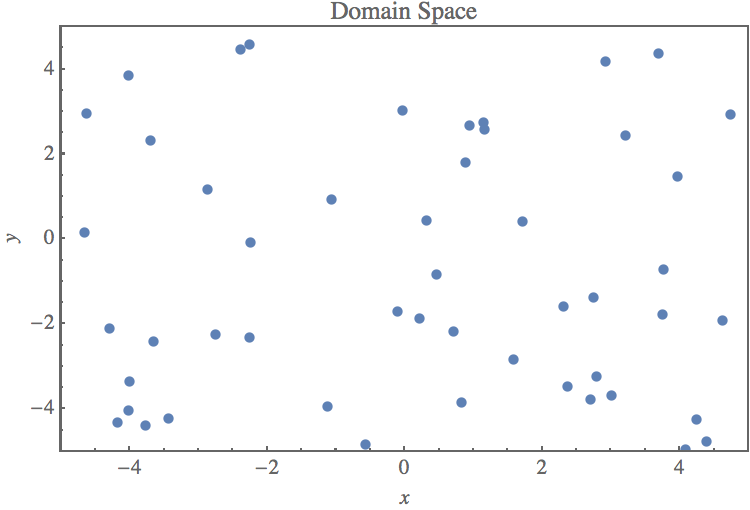
\includegraphics[height=0.25\textheight,width=0.5\linewidth]{../Plots/domainspace.png} &
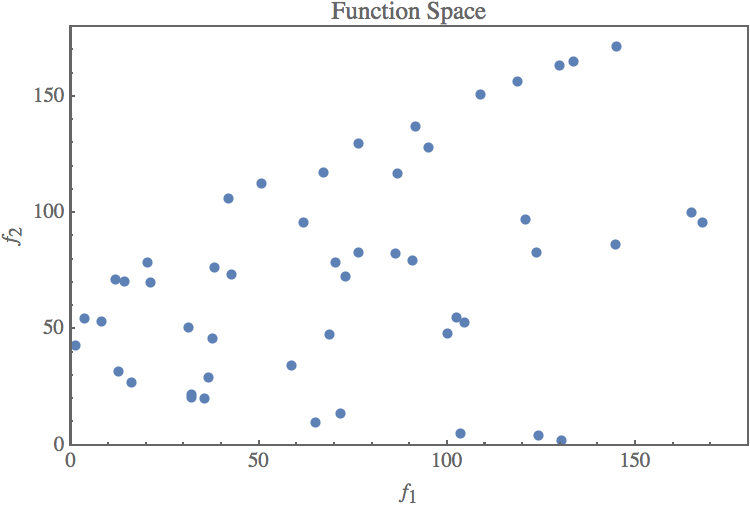
\includegraphics[height=0.25\textheight,width=0.5\linewidth]{../Plots/functionspace.png}
\end{tabular}
\end{table}

In a multi-objective problem, more often that not, the objectives will oppose each other; otherwise, the solution would be trivial. For example, when minimizing two objectives, a decrease in one objective would cause an increase in the other. This is known as tradeoff. When the objectives of one solution are more optimized than all of the objectives of another solution, then the former solution dominates the latter solution. If not all the objectives of a solution are more optimized, then the solutions are non-dominating.

Instead of a single solution, there are usually sets of solutions known as fronts. Fronts are sets of solutions in which every member of the set does not dominate other members of the set. Figure \ref{fronts} shows an example of a set of fronts for Equation \ref{binhkorn}. The most optimal front is known as the Pareto front, and finding the most optimal Pareto front is the goal of multi-objective optimization.
\begin{figure}[h!]
\begin{center}
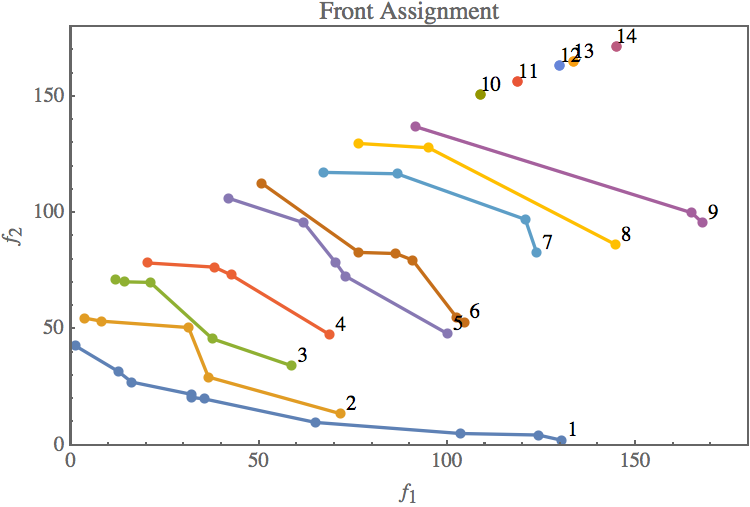
\includegraphics[height=0.35\textheight,width=0.7\linewidth]{../Plots/fronts.png}
\end{center}
\caption{Front assignment.} \label{fronts}
\end{figure}

\newpage
\section{Genetic Algorithms}
Genetic algorithms are a class of iterative optimization methods that use the principles of evolutionary biology. When referring to genetic algorithms, some of the terminology usually associated with optimization changes to the biological terms. Solutions in a multi-objective problem are referred to as individuals, and the set of individuals is known as a population. The fitness of an individual refers to the values of the objective functions. For example in Equation \ref{binhkorn}, the individual $(1,1)$ would have fitness values $(8,32)$. Each iteration in the genetic algorithm is called a generation. For some generation $n$, the $n$th population is known as the offspring population while the $n-1$th population is the parent population.

The genetic algorithm begins with some initial population and each generation afterwards produces an offspring population using genetic operators. Genetic operators include selection, crossover, and mutation. Genetic operators use the principle of natural selection to find the best solution while using the principle of diversity to avoid convergence to a local minima.

\subsection{Selection}
Selection operators are used to select which offspring survive to the next generation. Truncation is the simplest selection operator which simply chooses the fittest individuals from the parent and offspring population. Tournament selection is another selection operator that randomly sorts the individuals into blocks and chooses the best individual from each block.

\subsection{Crossover}
Crossover operators are used to mix two or more parents to produce similar, but slightly different offspring. Most crossover operators convert the indivudal into binary representation to perform the operations. One-point crossover crosses the binary digits at some crossover point of two parents to create two new individuals. For example, consider the parents 7 and 18 which in binary are 00111 and 10010 repsectively. Let the crossover point be position 3; thus the offspring would be 00010 and 10111 or 2 and 23 respectively. Another type of commonly used crossover operation is two-point crossover which is similar to one-point crossover but with two crossover points. Uniform crossover is a type of crossover in which each digit in the binary representation of the offspring is independently chosen from either parent with a fifty percent probability.

\subsection{Mutation}
Mutation operators are used to further preserve the diversity of a population to ensure nonconvergence to an optimum. A simple type of mutation involves the addition of a number chosen from some gaussian distribution, usually with a mean of 0 and a standard deviation of 1. Another type of mutation known as flip bit also performs operations on the binary representation of a number where each bit in the binary representation has some probability of being mutated.

\newpage
\section{Results}
A variety of functions were used to test a genetic algorithm code written in Fortran. The code begins by generating a uniformly distributed population. Then, the genetic operators of selection, crossover, and mutation were applied in that order to the population for each generation. The algorithm was run until a specified amount of generations. The default genetic operators were truncation selection, two-point crossover, and gaussian mutation. The crossover probability was fifty percent while the mutation probability was twenty percent.

\subsection{Operator Tests}
The Binh and Korn function is described in Equation \ref{binhkorn} and was used to test the crossover and mutation genetic operators. The population size was 100 and the algorithm was allowed to run for 10 generations.
\begin{table}
\caption{Crossover Results}
\label{crossover}
\begin{tabular}{cc}
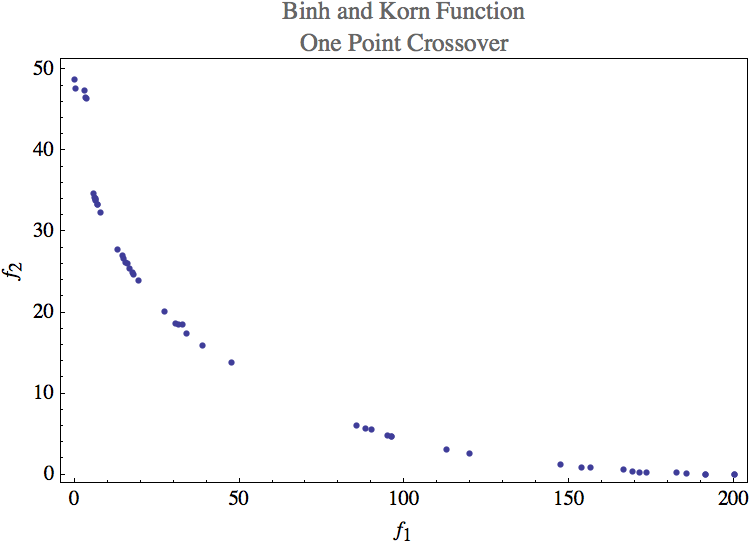
\includegraphics[height=0.25\textheight,width=0.5\linewidth]{../Plots/oneptcross.png} &
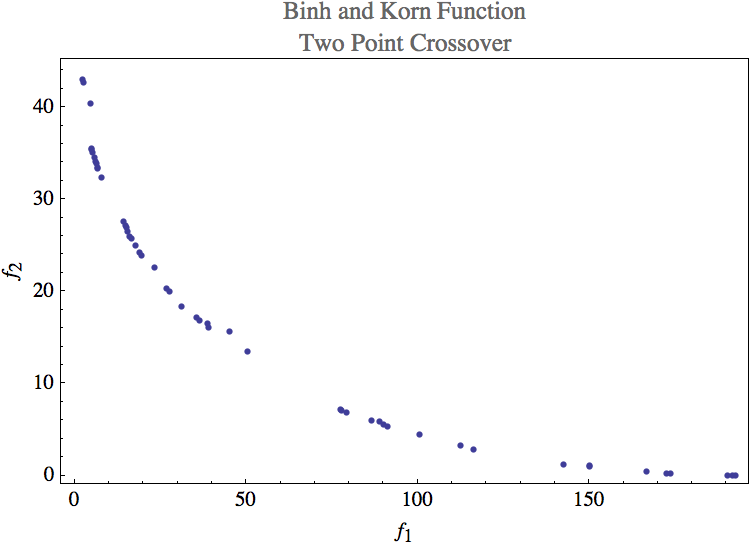
\includegraphics[height=0.25\textheight,width=0.5\linewidth]{../Plots/twoptcross.png} \\
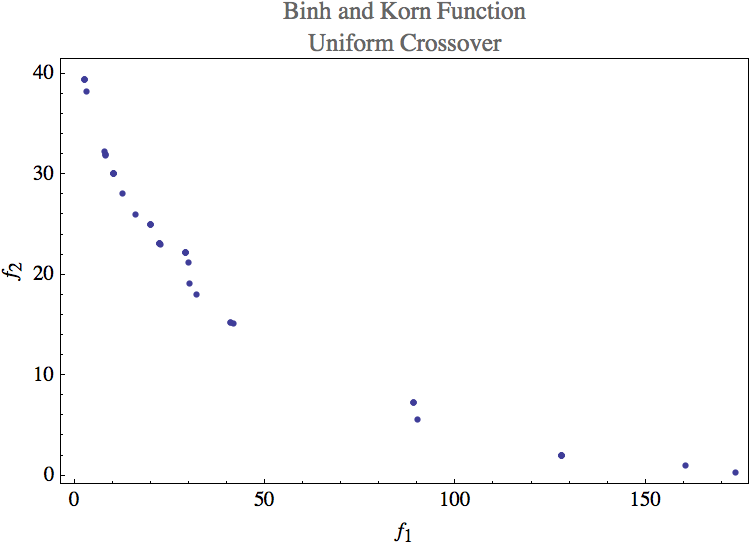
\includegraphics[height=0.25\textheight,width=0.5\linewidth]{../Plots/unifcross.png} &
\end{tabular}
\end{table}
Table \ref{crossover} compares the various crossover operators on the Binh and Korn function with the Gaussian mutation operator. Table \ref{mutation} compares the mutation operators on the Binh and Korn function with the two-point crossover.
\begin{table}
\caption{Mutation Results}
\label{mutation}
\begin{tabular}{cc}
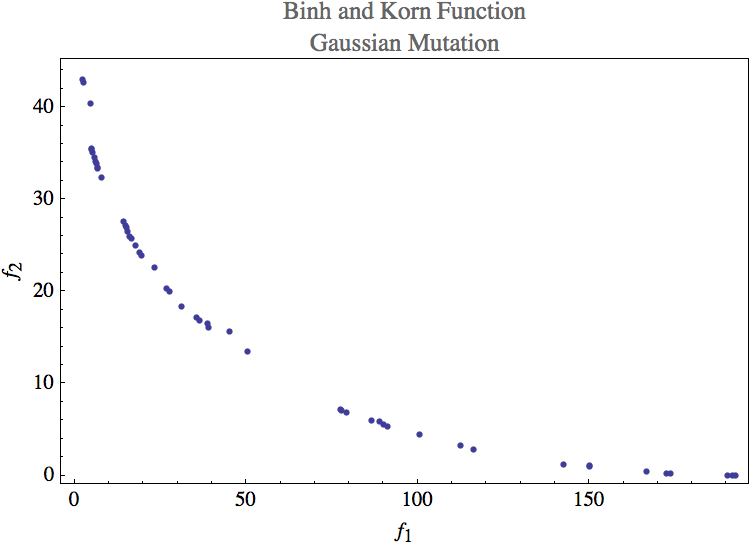
\includegraphics[height=0.25\textheight,width=0.5\linewidth]{../Plots/mutgauss.png} &
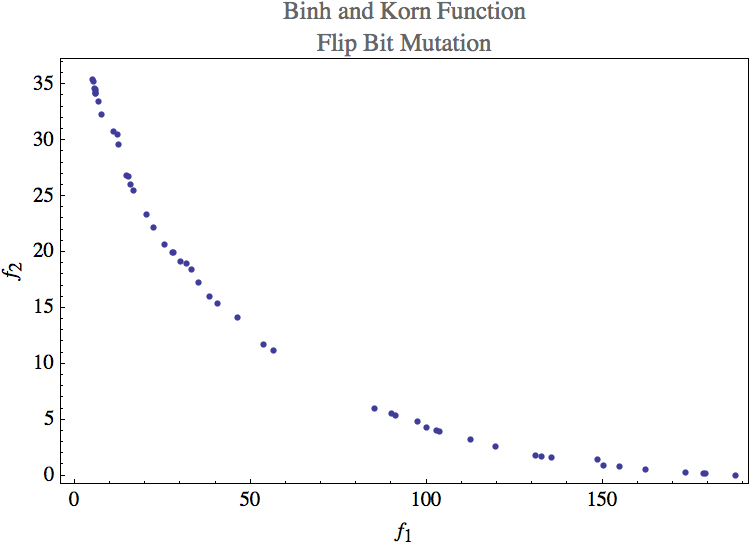
\includegraphics[height=0.25\textheight,width=0.5\linewidth]{../Plots/mutflipbit.png}
\end{tabular}
\end{table}

\subsection{Convergence Test}
The Ackley function as described in Equation \ref{test1} is a single-objective function used an example of genetic algorithms finding the global convergence. The population size was 50 and the algorithm was allowed to run for 5 generations.
\begin{equation}
\label{test1}
f\left(x,y\right)=-20\exp\left(-0.2\sqrt{0.5\left(x^2+y^2\right)}\right)-\exp\left(0.5\left(\cos\left(2\pi x\right)+\cos\left(2\pi y\right)\right)\right)+e+20
\end{equation}
Table \ref{ackley} shows the initial and final generation of solutions to the Ackley function. The function is shown by the surface while the points are the individuals in the population.
\begin{table}
\caption{Ackley Results}
\label{ackley}
\begin{tabular}{cc}
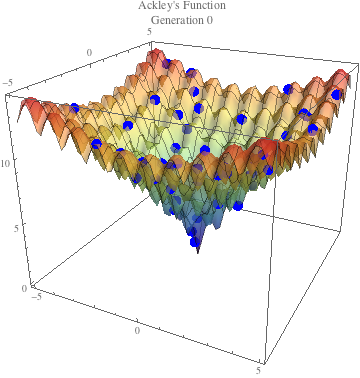
\includegraphics[height=0.4\textheight,width=0.5\linewidth]{../Plots/ackley0.png} &
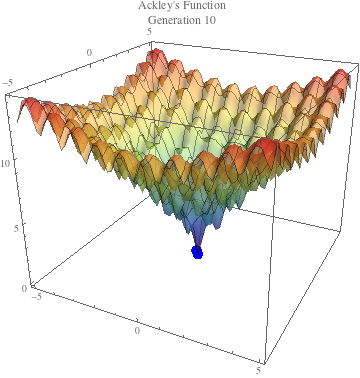
\includegraphics[height=0.4\textheight,width=0.5\linewidth]{../Plots/ackley10.png}
\end{tabular}
\end{table}

\subsection{Kursawe Function}
The genetic algorithm was finally used to optimize the Kursawe equation described in Equation \ref{test3}. The population size was 2000 and and the two-point crossover and gaussian mutation genetic operators were used. The algorithm was allowed to run for 20 generations.
\begin{equation}
\label{test3}
\textrm{Minimize}\begin{cases} 
    f_1(\pmb{x}) = \sum_{i=1}^2\left[-10\exp\left(-0.2\sqrt{x_i^2+x_{i+1}^2}\right)\right]\\
    f_2(\pmb{x}) = \sum_{i=1}^3\left(\left|x_i\right|^{0.8}+5\sin\left(x_i^3\right)\right)
  \end{cases}\\
\end{equation}
The first row of Table \ref{kursawe} shows the initial population while the second row shows the final population. The first column shows the full function space while the second column shows the function space zoomed into the final Pareto front of the solution.
\begin{table}
\caption{Kursawe Results}
\label{kursawe}
\begin{tabular}{cc}
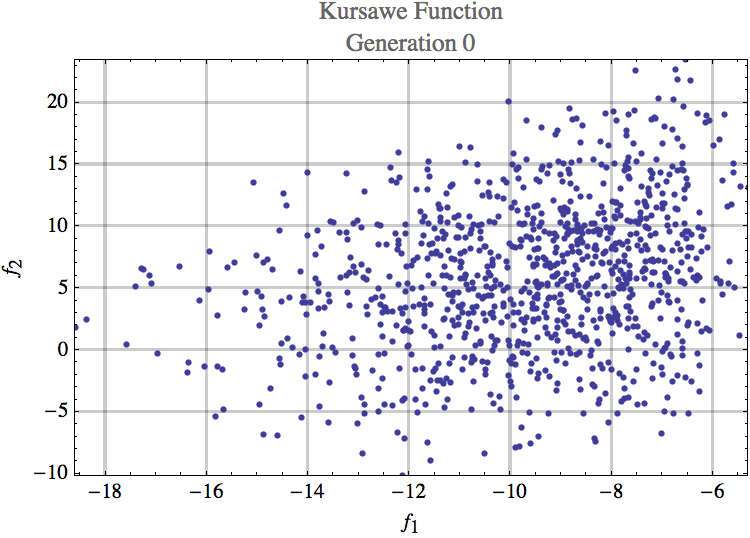
\includegraphics[height=0.25\textheight,width=0.5\linewidth]{../Plots/kursaweout0.png} &
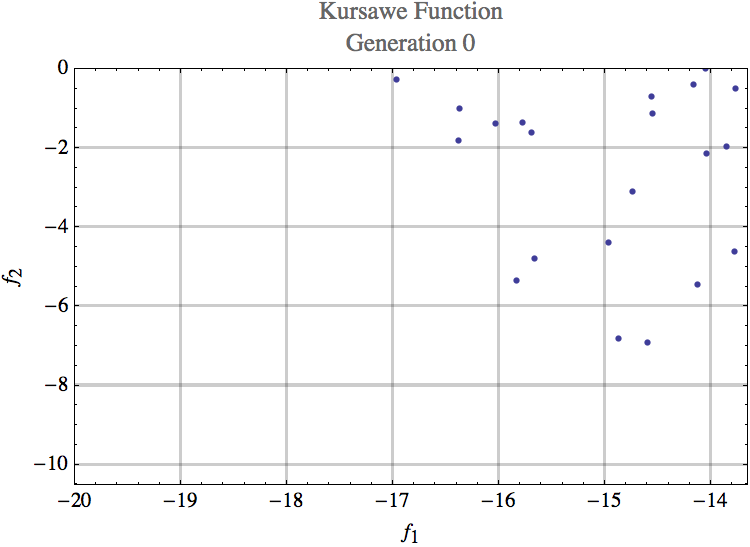
\includegraphics[height=0.25\textheight,width=0.5\linewidth]{../Plots/kursawein0.png}\\
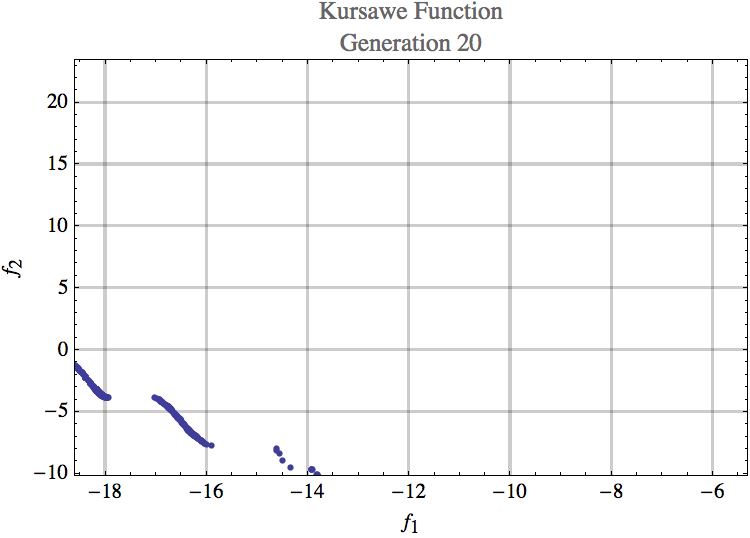
\includegraphics[height=0.25\textheight,width=0.5\linewidth]{../Plots/kursaweout20.png} &
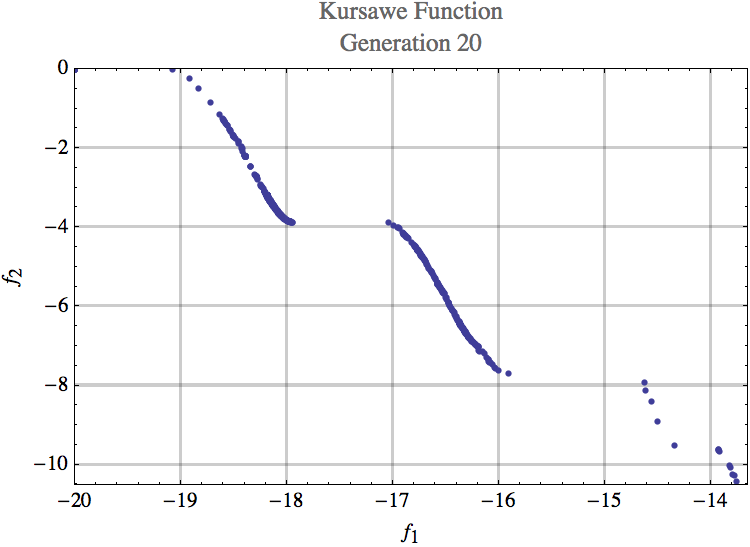
\includegraphics[height=0.25\textheight,width=0.5\linewidth]{../Plots/kursawein20.png}
\end{tabular}
\end{table}

\section{Conclusion}
The genetic algorithm code was successful in solving a variety of optimization problems. The genetic operators were successful in keeping diverse solutions along the Pareto front as opposed to converging to a single point along the Pareto front. The Ackley function has a clear global minimum at $(0,0)$ with multiple local minima surrounding it, but the genetic algorithm was still able to navigate the local minima to find the global minimum. Also, unlike the solutions for the Binh and Korn function, the solutions for the Kursawe function are not immediately obvious from the initial population. However, the genetic algorithm was able to converge to a solution that is clearly better than the initial solution.
\newline

\noindent Reference:

\noindent K. Deb, \textit{Multi-Objective Optimization using Evolutionary Algorithms} (John Wiley \& Sons, 2001).
\end{document}